\documentclass[conference]{IEEEtran}
\IEEEoverridecommandlockouts
% The preceding line is only needed to identify funding in the first footnote. If that is unneeded, please comment it out.
%Template version as of 6/27/2024

\usepackage{amsmath,amssymb,amsfonts}
\usepackage{algorithmic}
\usepackage{graphicx}
\usepackage{textcomp}
\usepackage{xcolor}
\usepackage{hyperref}
\usepackage{listings}


\begin{document}
\title{Comparison and Implementation of Packet Scheduling Methods}

    \author{
        \IEEEauthorblockN{Ethan Ruchotzke}
        \IEEEauthorblockA{
            CprE 558 \\
            \textit{Dept. of Computer Engineering} \\
            \textit{Iowa State University}\\
            Ames, Iowa \\
            ethanr@iastate.edu
        }
    }

    \maketitle

    \begin{abstract}
        Real time networks are an important part of supporting communication between time-sensitive applications.
        However, the current iteration of the Internet does not, by default, support strict requirements for routing (best
        effort model).
        This project investigates one aspect of real-time networking, packet scheduling.
    \end{abstract}

    \begin{IEEEkeywords}
        real-time, scheduling, networking, latency, fairness
    \end{IEEEkeywords}

    \section{Introduction}
    Traditionally, in the current Internet, we are spoiled by the ability to get a packet from any device to another device.
    Using the current model, I am able to send a packet out, via devices I don't own, and get a response from a device across the
    world in less than a second.
    However, as astonishing as that is from a human perspective, it is not always enough.
    Some applications that are time sensitive, known as real-time applications, rely on firm guarantees of timing.
    The current model of the Internet is based on best-effort; it works most of the time, but makes no comments about packet
    loss or latency.
    This is not acceptable for time-sensitive applications, which may need strict guarantees on performance
    to maintain safety.

    As stated above, safety is one major part of time-sensitive applications.
    For example, imagine a factory being controlled
    via electronic devices.
    In the event a control command is coming from the Internet, a short delay may be needed to ensure
    a dangerous industrial process remains controlled, or a car remains on the road.
    We don't want a factory's vital control
    loop to be interrupted or delayed by congestion caused by a popular meme.
    For that reason, specific protocols are used
    to support an overlay network of real-time routers, capable of making more controlled guarantees about timing and resources
    over a network.

    Real-time networks are a broad subject area.
    Essentially, all of networking has to be thought about more deeply in a real-time context.
    Real-time LAN studies how local networks (Ethernet, CAN, etc.) can be adapted/built to work in a time-sensitive environment.
    Real-time WAN, on the other hand, studies how inter-network communication can be done in a time sensitive manner.
    Naturally, real-time WAN has a large number of sub-problems, like shaping traffic to make it behave better and
    how to schedule packets to get optimal performance and ordering (based on some metric) when routing packets.

    This project sought to implement and investigate the final part of real-time WAN; the scheduling of packets.
    Scheduling is an interesting and rich area, and based on the work done in class alone, there were a large number
    of project options.
    Scheduling is both easily implementable and easily quantifiable, and made a perfect topic for more investigation.

    \section{Project Objectives \& Scope}
    This section will provide a definition of the exact questions I sought to answer through this project.
    I will begin by defining where this problem has value, and then further define the objectives and scope of this project.

    \subsection{System Model}
    In the context of a real network, packet scheduling happens on any routers carrying real-time flows.
    For example, if
    two different devices share a router, and both require real-time guarantees, packet scheduling is used on their connected
    router to properly order packets.
    This process is replicated on any routers responsible for handling real-time flows.

    This is relevant to any type of device requiring real-time flows.
    Typically, this would be required by an application requiring strict flows, running on any type of device (microcontroller
    or regular computer).
    IoT devices may utilize scheduling to most efficiently route traffic, whereas a regular, heavier duty application may
    require timing or latency constraints, like VOIP or control applications.

    \subsection{Problem Statement}
    As this project focuses on packet scheduling, the problem is simple to define.
    The problem with more advanced routing algorithms is that they're often difficult to characterize, unlike traditional
    single-queue systems.
    Because of this, extra work is required to validate and verify the performance of these algorithms.

    One interesting way of doing this is through utilization of formal methods.
    In 2023, a team from the University of Waterloo (collaboration with Microsoft)~\cite{arashloo_formal_2023} utilized formal verification to compare
    a given routing scheme (queues and management) against a set of constraints.
    This allowed the team to exhaustively search all possible packet transmissions for packet series which caused the algorithm
    to fail against some metric and constraint.
    While a more perfect method than others, formal methods requires more modeling and setup time, which is a turnoff to people
    looking for quick, but generally correct, results.

    The other more common method, which I investigated, was simulation.
    Simulation of networks is fairly straightforward,
    and as I'll mention in the future, there are many solutions available.
    Through simulation, one can define a set of packet flows and implement a route discipline (how queues are managed) and
    get explicit results back on how the flows performed.
    This was the focus of my project.
    I defined three algorithms (FIFO, Round Robin, and Fair Queueing) and compared them with respect to metrics I could simulate.

    \subsection{Objectives and Scope} \label{subsec:obj_scope}
    I broke my general project of interest into a few specific objectives:

    \begin{itemize}
        \item Implement a few schedulers (FIFO, Round Robin, Fair Queueing) within a network simulator
        \item Create a test load to utilize for metrics
        \item Verify performance against a few metrics:
        \begin{itemize}
            \item Latency (impact of scheduling on delay)
            \item Fairness (are loads being treated equally, or proportional to weight?)
        \end{itemize}
    \end{itemize}

    Originally, this was intended to be the entirety of the project.
    However, as discussed in the next section, I was displeased with the current state of network simulation.
    To remedy this, I added a fourth objective to my project:
    \begin{itemize}
        \item Implement a basic network simulator capable of easily investigating scheduling.
    \end{itemize}

    While not necessarily relevant to scheduling itself, it became apparently that something more useful was needed.
    Again, this will be explained in the following section.

    That is also the total scope of this project; the following questions are interesting, but were not investigated for
    this project.

    \begin{itemize}
        \item Can we formally prove a scheduler is fair?
        \item How does crosstalk between flows impact latency?
        \item Investigation of other metrics, like utilization, jitter, and acceptance rate.
    \end{itemize}

    These topics would make an interesting set of future works to investigate, but for now, the original vision stood.

    \section{Solution Methodology / Approach} \label{sec:approach}
    The approach to this research project is simple; develop a simulation capable of measuring the impact of schedulers
on specified packet flows.
    This ended up being a large part of the project, as my initial goal was not easily realizable
in a tool like NS-3.
After a simulation was planned, a specific experimental approach was decided upon.
This section will detail the decision-making which happened, and culminate in a scenario which demonstrates the ideas
I was intending to convey.

    \subsection{Simulation Methodology}
I began by looking at various network simulators, as my goal was to simulate networks.
I settled on three initial choices: NS-3, GNS3, and Mininet.
After investigating all three, I realized they all had the basic capabilities I needed; emulation of a network to gather
statistics from.

I began by eliminating choices.
The first to be eliminated was GNS3.
I had used the tool in the past and really liked it, however for this experimentation it was overkill.
GNS3 provided a front-end and GUI for what was essentially a set of virtual machines.
While excellent for other things, it was far too much for what I needed here.

I then did some investigation into Mininet.
Mininet was more closely aligned with what I sought; it didn't use a GUI or have a lot of bloat, and it allowed for
network simulation within a code environment.
However, as I dug into the differences between Mininet and NS-3 more, I realized Mininet was also not what I sought.
Mininet focused on software-defined networking and other pieces of the puzzle; it also had VM integration, which was again
for more complicated than I was seeking.

This left me with NS-3, which was originally a perfect choice.
NS-3 was great because it didn't utilize VMs, it essentially simulated everything from a single C++ program.
However, after a couple of days of working with it, I realized it was focused more on the networking than the routing.
While it gave me the tools I needed, I simply wasn't able to get the things I needed (modification of the IP stack) done
in a reasonable amount of time, and so I abandoned it.

This left me with a final option; writing my own simulation.
I have a lot of experience writing simulations, and am quite experienced with networking, so I was able to construct my own
network simulator fairly quickly.
I found a useful discrete-event simulation library, SimPy, to run the simulation under the
hood.
More will follow on the simulation architecture (and why it is valid) in the implementation section.

    \subsection{Experimental Approach}
I specifically identified two properties I wanted to investigate: fairness and latency.
This had an impact on my choice of simulation target.

The first obvious constraint would be the bandwidth of the input and output.
To measure the impact of congestion on the performance, I would need three scenarios.
One scenario would have significantly lower bandwidth on the output link, representing a congested network.
Another needs to have equal bandwidth, meaning that the queues should be constantly moving forward.
Finally, the last would need greater bandwidth than required, to measure the pure impact of the scheduling algorithm on latency.

However, outside of these constraints, the network was simple to design.
\begin{itemize}
    \item Multiple input flows (of equivalent bandwidth) to check fairness of
    \item One router to implement scheduling on
    \item One server to measure results with
\end{itemize}

Thus, a simple linear network with three inputs was used.

    \subsection{Example Scenario}
The scenario in question has a layout which resembles that of figure~\ref{fig:test-net}.

\begin{figure}[htbp]
    \centering
    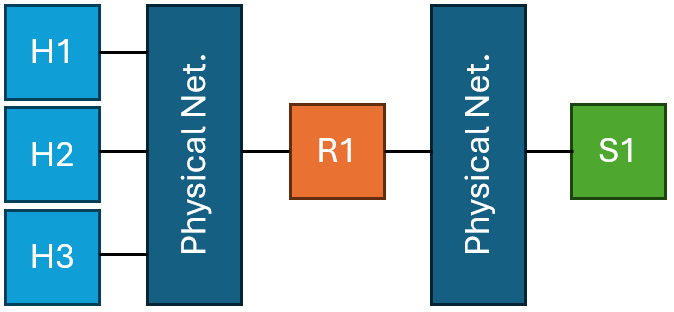
\includegraphics[width=0.4\textwidth]{../img/test-network}
    \caption{The test network.}
    \label{fig:test-net}
\end{figure}

Three hosts generate packet flows which are reserved on router 1 (R1). Each host has an application which demands
an equivalent bandwidth, but with different packet rates. Each host requires 100b/s, however:
\begin{itemize}
    \item Flow 1 sends 100 byte packets every second
    \item Flow 2 sends 20 byte packets every 0.2 seconds
    \item Flow 3 sends 200 byte packets every two seconds
\end{itemize}

In this way, the router can have a measurable impact on output, as each flow is different.

This could be equivalent to a multi-tier network.
Flow 2, with frequent packets, may represent an IoT device sending sensor values into a network (many small updates).
Flow 1 has less, but larger packets; it would be equivalent to a device collecting multiple packets into one larger update.
Finally, Flow 3 takes that to the extreme, collating even more information.
Each flow has identical bandwidth needs, but has different packet rates.

Using this example, I was able to successfully implement packet routing disciplines and measure their impact on received traffic.

    \section{Implementation / Simulation Architecture} \label{sec:impl}
The following section will go into the technical detail of the platform I developed, how the schedulers being tested were
implemented, and how results were measured.

    \subsection{Simulator Implementation}
As mentioned earlier, I opted to create my own simulation, as I felt I had both the expertise and programming knowledge
to successfully model the system.
The most important aspect was thinking about the travel of packets; how things were delayed
and how networks were accessed.
My simulation brings together a handful of important variables (bandwidth, CSMA-CD replication, and network stacks) to
attempt to faithfully model a real network without the overhead of a larger simulator.

The simulator itself is built on a discrete event simulation environment, called SimPy.
SimPy is built around the idea of generators, or functions which generate events and can await as needed.
For example, an ICMP echo client is simple to implement as a generator, as it periodically generates packets and can
await responses.
The basic building block of a generator is extendable and used to build all the important components.

Also important were queues and resources, both of which this underlying library had built in.
These allowed for modeling queues (with latency) between parts of the network stack and also to provide CSMA-like access
to the simulated network.

The simulation is built using four major components: Networks, Nodes, Network Stacks, and Applications.

    \subsubsection{Networks}
Networks are modeled as simple LAN environments connecting together multiple devices.
Networks have two properties: bandwidth (how many bytes can be sent per second) and the shared resource.
Bandwidth was important to model, as it has an impact on delays experienced by packets.
Simply put, a delay for a packet is experienced because of bandwidth, proportional to the packet size.
A larger packet will always take longer to transmit into a network.
Once transmitted, all connected devices receive a copy of the packet, and need to do any filtering themselves.
A benefit of bandwidth is that it can be sampled; every 1000th of a second, a monitor polls the network to see if it is
active.
If the network is active, that can be factored into bandwidth utilization.
While not useful as a measure for this project, it could be useful later.

The shared resource of the network is used to model CSMA.
If many devices are competing for access to the local network, that has an impact on delay, and so needed to be modeled.
To do this, a mutex was utilized to restrict the number of transmitting nodes to one.
This was made very easy with the SimPy library, and added an extra level of realism to the simulation.

    \subsubsection{Nodes}
A node is the basic building block of the simulation.
Each node represents a single device, like a computer, IoT device, or server.
Nodes are incredibly simple; they essentially contain a single network stack, which will be discussed in the next section.

    \subsubsection{Network Stack}
The network stack is the brain of the simulation; each node has at least one set of layers, which combined make a stack.
The network stack is divided into three "layers": an Ethernet layer, an IP layer, and an Application layer.
Each layer has a specific purpose, and is analogous to its corresponding real-world equivalent.
Some devices may only have a single "stack": these would correspond to host/server devices, which are only connected to one LAN.
In contrast, other devices may have multiple "stacks", in this case referred to as interfaces.
These devices are the routers of the simulation.
A visual of the layers can be found in figure~\ref{fig:combo}.

\begin{figure}[htbp]
    \centering
    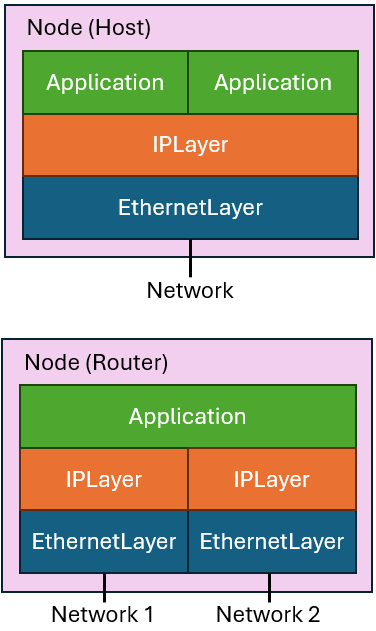
\includegraphics[width=0.3\textwidth]{../img/combo}
    \caption{The architecture of a host and a router.}
    \label{fig:combo}
\end{figure}

Queues are used between layers of the stack.
Like real-world components, the speeds of each layer are not immediate, and delays
are included to represent the processing time of each layer.
This also allows for more intricate queue handling, like the goal of this project was to investigate.

The Ethernet layer is the device directly connected to a LAN.
The network address is an Ethernet address.
This layer receives/listens for all traffic on the LAN and filters it accordingly.
If relevant, it forwards the packet up to the IP layer.

The IP layer is the important part of the simulation; it is used to route across multiple LANs.
An IP address is used to identify the device at this layer; again, filtering is used.
If the filter matches, the packet is forwarded to an application.
If the filter does not match, the packet is discarded (if not a router) or checked against a route table for forwarding.
In our case, the extra important piece is the discipline: the discipline is the scheduler for packets arriving at the IP layer.
For normal devices, the scheduler is a simple FIFO queue, though for the router itself, different flows receive different
queues.

A tangential note: routing is performed statically.
After configuring the network, a helper function is called.
This automatically fills all ARP tables with local IP/HW address mappings to facilitate local communication.
Basic route tables are then constructed for all interfaces, where direct connections are generated.
Currently, a more advanced routing system (like precomputed source routing) is not available.

Finally, the application layer is responsible for generating and receiving packets.
This is where the simulation events are driven; some applications (clients) generate traffic, while others (servers)
consume and document it.
More about applications will follow in the next section.

    \subsubsection{Applications}
Applications are responsible for the generation and logging of packets.
This is the driver of the whole simulation (setting up flows) but also for the monitoring (logging received packets).
In my simulation, I designed two applications.

The first is the generator, which is like a variable size/rate ICMP echo client.
The generator is provided three arguments.
The first is a target; this simply tells the packets where they are being sent.
Then, a rate is provided; this tells the generator how fast to attempt to send packets (queue them at the IP layer if sent too fast).
Finally, a size is provided; this gives the size of the packet sent at the given rate.
Using these arguments, we essentially have a traffic generator with configurable bandwidth.

The second is the logger server, which does as its name suggests: it logs arriving packets.
This is useful as we can compute many properties from a simple log.
Each arrival time is documented, along with source, send time, and size; this information is saved to a CSV.
From these raw values, most important properties can be computed, like latency, jitter, fairness and more.

    \subsection{Scheduler Implementation}
The core of the implementation for this project was the implementation of the packet schedulers; alternatively, I referred
to these as disciplines, as they were different ways of scheduling packets.
The schedulers lie within the implementation of the IP layer.
A scheduler is straightforward: packets are enqueued to it, and it decides how to dequeue packets from its input queues.

Scheduler implementation is based around two functions:
\begin{itemize}
    \item $enqueue\_packet$
    \begin{itemize}
        \item Enqueues a supplied packet to one of the input queues.
    \end{itemize}
    \item $proc\_handle\_disc$
    \begin{itemize}
        \item The process used to handle moving an item to the output
    \end{itemize}
    \subsection{Measurement Implementation}
\end{itemize}

Schedulers are defined with an initial set of "flows" (IP-address matched queues) along with a default queue.
As packets are enqueued, they are sorted into one of these flows.

Dequeueing the packet is a bit more complicated.
Important here is the fact that we want to wait until the Ethernet layer demands a packet to supply one.
This is because we're interested in the timing/behavior of the scheduler under load.
If we simply immediately dequeue packets when available, our scheduler will never fill up, and never utilize advanced
behaviors.
To accomplish this, we simply wait until the Ethernet layer's input queue is empty before dequeueing a packet into it.

The pseudocode for the algorithms has been provided in two figures.
The round robin pseudocode can be found in figure~\ref{fig:rr_impl}, and the fair queue pseudocode can be found in
figure~\ref{fig:fq_impl}.
Note that FIFO was implemented as a round robin queue with zero flows (so all packets went to a default queue).
This is merely pseudocode; to see the full implementation, check out my open-source \href{https://github.com/Ruchotzke/558-final}{GitHub repository}.

\begin{figure*}[tbp]
    \begin{lstlisting}
    handle_rr():
        While True:
            # Check the output queue and make sure it is empty (on-demand dequeue)
            if output_queue.items == 0:
                # Iterate through all queues, starting from the last we emptied
                for i in range(0, flows):
                    j = (i + prev_pos) % len(flows)
                    if flows[j] is not empty:
                        dequeue from flow j
                        save position
            # Poll Delay
            wait 0.001s
    \end{lstlisting}
    \caption{Round Robin Implementation}
    \label{fig:rr_impl}
\end{figure*}

\begin{figure*}[tbp]
    \begin{lstlisting}
    enqueue_packet(pkt):
        # Find the corresponding flow
        flow = matching_flow(pkt)

        # Handle finish time
        vir_start = max(self.virt_time, flow.vir_finish)
        pkt.finish_time = pkt.len + vir_start
        flow.vir_finish = pkt.finish_time
        flow.enqueue(pkt)

    handle_fq():
        While True:
            # Check the output queue and make sure it is empty (on-demand dequeue)
            if output_queue.items == 0:
                # Find the packet with the next smallest finish time
                min_finish = infinity
                for each flow:
                    if flow[0].finish_time < min_finish:
                        save flow

                # If we found a flow (queues may be empty) dequeue and update virt time
                if flow is not null:
                    dequeue flow[0]
                    virt_time = max(virt_time + flow[0].len, flow[0].finish_time)
            # Poll Delay
            wait 0.001s
    \end{lstlisting}
    \caption{Fair Queue Implementation}
    \label{fig:fq_impl}
\end{figure*}


    \section{Evaluation}
    \subsection{Experiment Setup}

    \subsection{Results}

    \subsubsection{Fairness}

    \subsubsection{Latency}

    \section{Conclusions}

    \section{Self Assessment}
    See self assessment in table~\ref{tab:self-assmt}.

    \begin{table*}[b]
        \centering
        \caption{Self assessment table.}
        \label{tab:self-assmt}
        \begin{tabular}{|c|c|c|}
            \hline
            \textbf{Project Learning Objectives} & \textbf{Status} & \textbf{Pointers in the document} \\
             & (Not/Partially/Mostly/Fully Completed) &  \\
            \hline
            Self-contained description of the project goal, scope, and requirements & Fully Completed & Subsection~\ref{subsec:obj_scope} \\
            \hline
            Self-contained description of the solutions & Fully Completed & Section~\ref{sec:approach} (entire section)\\
            \hline
            Adequate description of the implementation details & Fully Completed & Section~\ref{sec:impl} (entire section)\\
            \hline
            Testing and evaluation - test cases, metrics, performance & Fully Completed & \\
            \hline
            Overall project success assessment & Fully Completed & \\
            \hline
        \end{tabular}

    \end{table*}

    \section{References}
    \bibliographystyle{ieeetr}
    \bibliography{558}


\end{document}
